\documentclass{ximera}  


\input{../preamble.tex}



 
\title{Types of Transmission Lines} 
\author{Milica Markovic} 
\outcome{Name several transmission lines.}
\begin{document}  
\begin{abstract}  

\end{abstract}  
\maketitle    






Any wire, cable, or line that guides energy from one point to another
is a transmission line. Whenever we make a circuit on a breadboard,
every wire attached forms a transmission line with the ground wire. Whether we see the propagation (transmission line) effects on the
line depends on the line length, and the frequency of the signals used. 
At lower frequencies or short line lengths, we do not
see any difference between the signal's phase at the generator and the load,
whereas we do at higher frequencies.








\section{Types of transmission lines}

\begin{enumerate}
\item Coaxial Cable, Figure \ref{fig:qm/Coax}
\item Microstrip, Figure \ref{fig:qm/MStrip}
\item Stripline, Figure \ref{fig:qm/Strp}
\item Coplanar Waveguide, Figure \ref{fig:qm/CPW}
\item Two-wire line, Figure \ref{fig:qm/TwoWL}
\item Parallel Plate Waveguide, Figure \ref{fig:qm/PPW}
\item Rectangular Waveguide, Figure \ref{fig:qm/RecWG}
\item Optical fiber, Figure \ref{fig:qm/OF}
\end{enumerate}




\begin{figure}[ht!]
\begin{center}
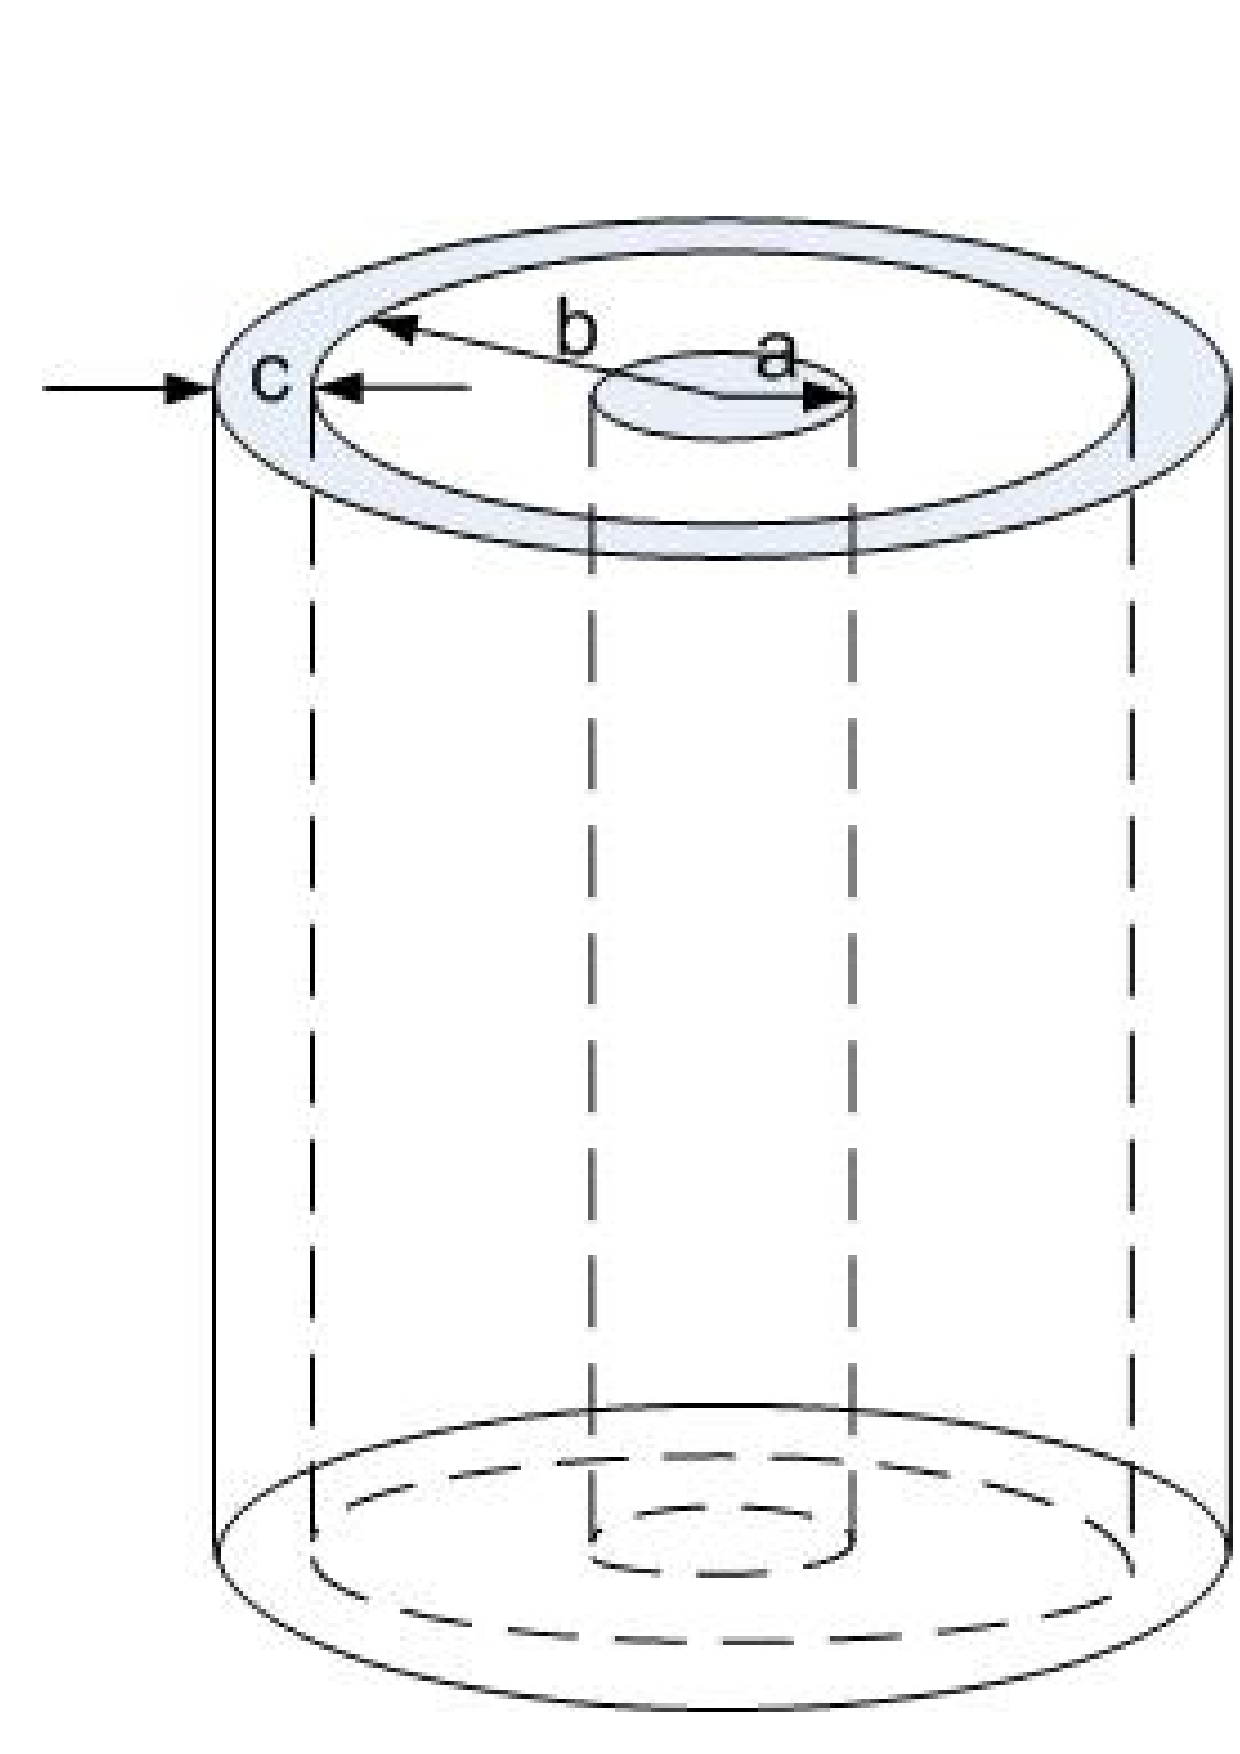
\includegraphics[scale=0.4]{../jpg/coax.jpg}
\caption{\label{fig:qm/Coax} Coaxial Cable}
\end{center}
\end{figure}


\begin{figure}[ht!]
\begin{center}
\includegraphics[scale=0.4]{../jpg/microstrip.jpg}
\caption{\label{fig:qm/MStrip} Microstrip}
\end{center}
\end{figure}

\begin{figure}[ht!]
\begin{center}
\includegraphics[scale=0.4]{../jpg/stripline.jpg}
\caption{\label{fig:qm/Strp} Stripline.}
\end{center}
\end{figure}

\begin{figure}[ht!]
\begin{center}
\includegraphics[scale=0.4]{../jpg/cpw.jpg}
\caption{\label{fig:qm/CPW} Coplanar Waveguide.}
\end{center}
\end{figure}

\begin{figure}[ht!]
\begin{center}
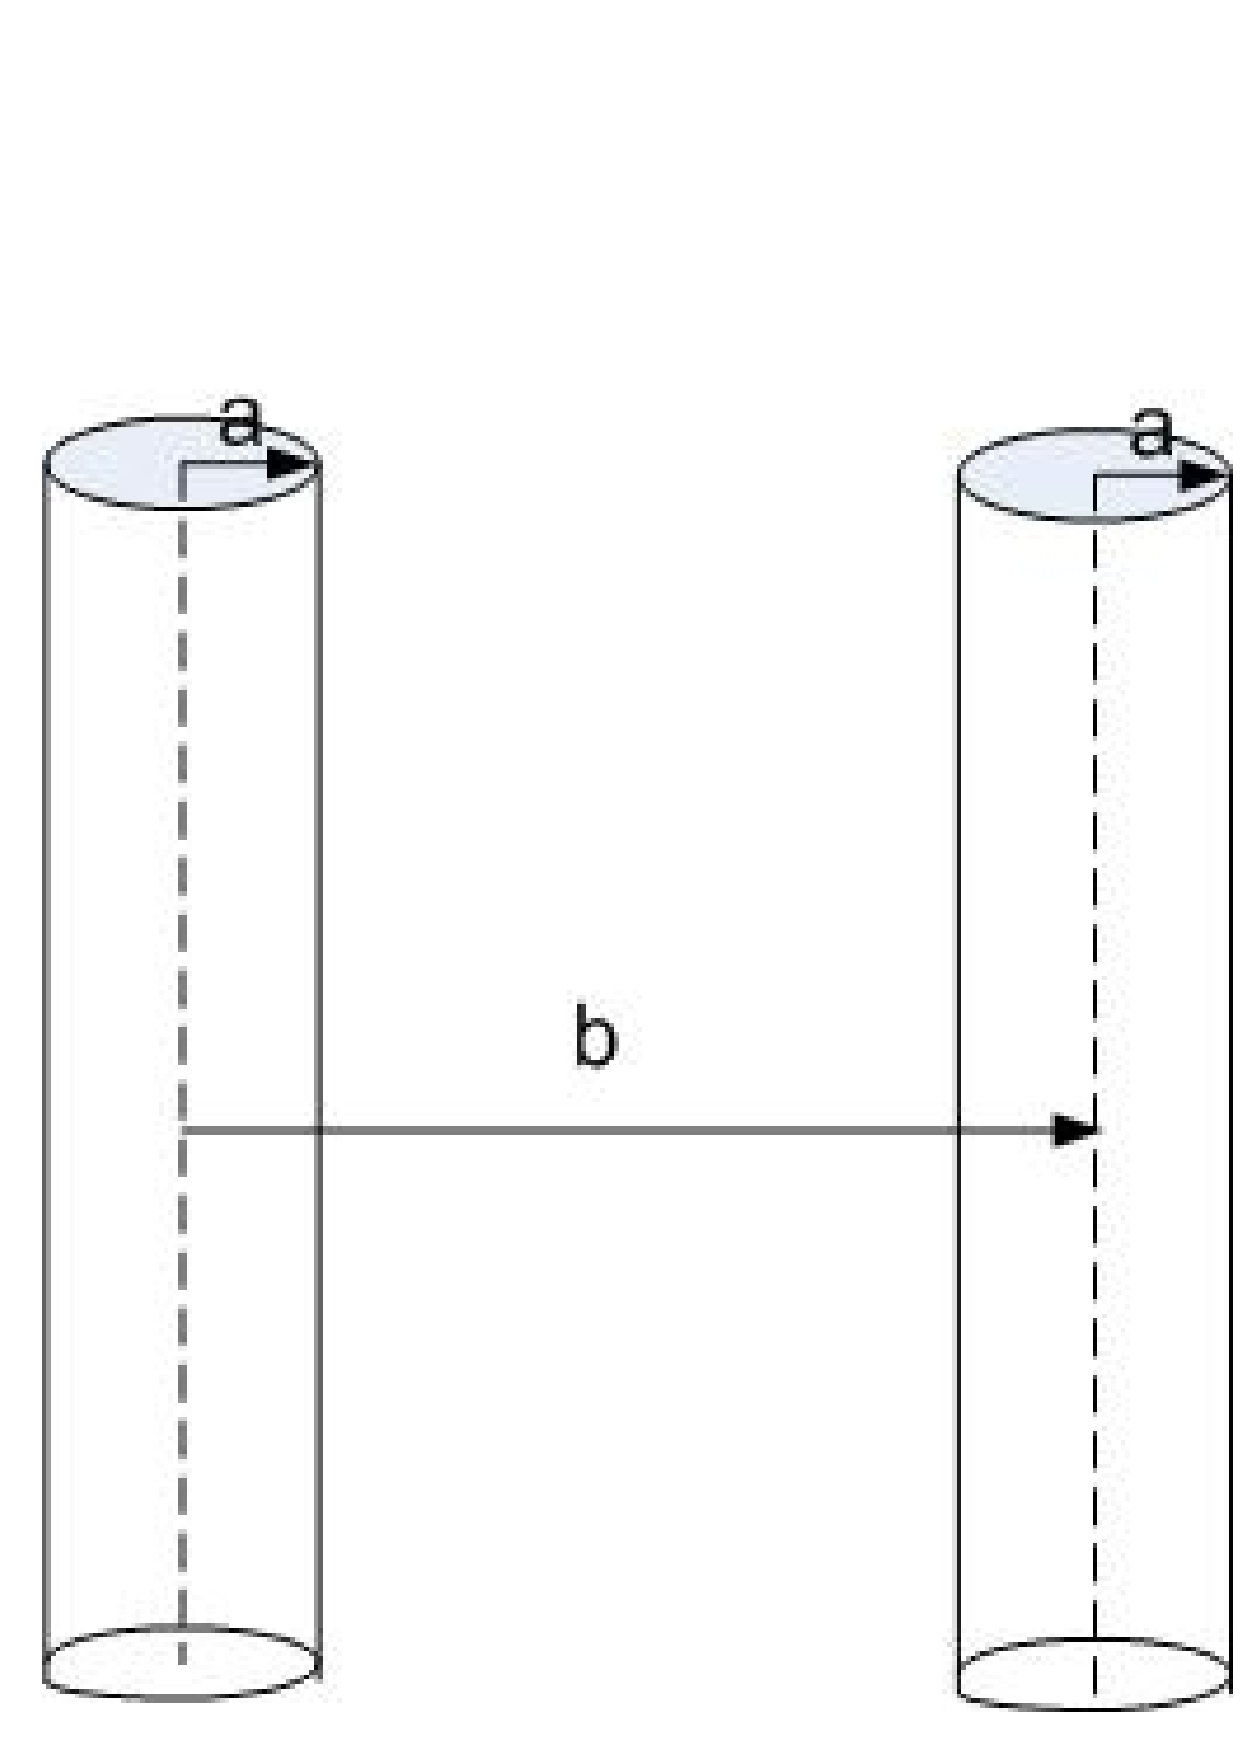
\includegraphics[scale=0.4]{../jpg/twowireline.jpg}
\caption{\label{fig:qm/TwoWL} Two-wire line.}
\end{center}
\end{figure}

\begin{figure}[ht!]
\begin{center}
\includegraphics[scale=0.4]{../jpg/ppw.jpg}
\caption{\label{fig:qm/PPW} Parallel-Plate Waveguide.}
\end{center}
\end{figure}

\begin{figure}[ht!]
\begin{center}
\includegraphics[scale=0.4]{../jpg/rectwg.jpg}
\caption{\label{fig:qm/RecWG} Rectangular Waveguide.}
\end{center}
\end{figure}

\begin{figure}[ht!]
\begin{center}
\includegraphics[scale=0.4]{../jpg/fiber.jpg}
\caption{\label{fig:qm/OF} Optical Fiber.}
\end{center}
\end{figure}


\section{Propagation modes on a transmission line}

Coax, two-wire line, transmission line support TEM waves. Waves on microstrip lines can be approximated as TEM up to the 30-40\, GHz (unshielded), up to 140\,GHz shielded.




\begin{enumerate}
\item Transversal Electro-Magnetic Field (TEM). Electric (E), and Magnetic (M) fields are entirely transversal to the direction of
propagation
\item Transversal Electric field (TE), Transversal Magnetic Field (TM),  M or E field is in the direction of propagation
\end{enumerate}

Transmission lines we will discuss in this course carry TEM fields.

%\begin{center}  
%\youtube{0aQpLSu2fMs}  
%\end{center}



\end{document} 
